\documentclass{article}
\usepackage{graphicx}
\usepackage{wrapfig}
\usepackage{subcaption}
\usepackage[margin=1in]{geometry}
\usepackage{amsmath} % or simply amstext
\usepackage{siunitx}
\usepackage{booktabs}
\usepackage[export]{adjustbox}
\newcommand{\angstrom}{\textup{\AA}}
\newcommand{\colormap}{jet}  % colorbar to use
\usepackage{cleveref}
\usepackage{booktabs}
\usepackage{gensymb}
\usepackage{float}

\renewcommand{\thefigure}{S\arabic{figure}}
\renewcommand{\thesection}{S\arabic{section}}
\renewcommand{\thepage}{S\arabic{page}}
\renewcommand{\thetable}{S\arabic{table}}

\title{Supporting Information: The Transport Mechanisms of Polar Solutes in a Cross-linked H\textsubscript{II} Phase Lyotropic Liquid Crystal Membrane}
\author{Benjamin J. Coscia \and Michael R. Shirts} 

\begin{document}

  \maketitle
  \graphicspath{{./supporting_figures/}}
  \bibliographystyle{ieeetr}

  \section{Setup and analysis scripts}\label{section:python_scripts}

  All python and bash scripts used to set up systems and conduct post-simulation trajectory
  analysis are available online at \texttt{https://github.com/shirtsgroup/LLC\_Membranes}.
  Documentation for the \texttt{LLC\_Membranes} repository is available at 
  \texttt{https://llc-membranes.readthedocs.io/en/latest/}. Table~\ref{table:python_scripts}
  provides more detail about specific scripts used for each type of analysis performed in
  the main text.
  
  \begin{table}[htb!]
  \centering
  \newcolumntype{A}{ >{\centering\arraybackslash} m{2.5in} }
  \newcolumntype{B}{ >{\centering\arraybackslash} m{0.75in} }
  \newcolumntype{C}{m{2.75in}}
  \begin{tabular}{|A|B|C|}
  \hline
  \textbf{Script Name} & \textbf{Section} & ~~~~~~~~~~~~~~~~~~~~~\textbf{Description} \\
  \hline

  \texttt{/setup/param.sh} & TBD & Parameterize liquid crystal monomers and 
  solutes with GAFF \\ \hline

  \texttt{/setup/solvation\_equilibration.py} & TBD & Add water to the pores and tails
  in order to achieve a specific total water content and ratio of water molecules in each
  region, then equilibrate the solvated system. \\ \hline
  
  \texttt{/setup/input.py} & TBD & Create GROMACS topology and .mdp files \\ \hline
  
  \texttt{/setup/xlink.py} & TBD & Iteratively cross-link a configuration \\ \hline
  
  \texttt{/setup/place\_solutes\_pores.py} & TBD & Place a desired number of solutes
  in the pore center, equally space in the $z$-direction. \\ \hline
  
  \texttt{/analysis/msd.py} & TBD & Calculate the mean squared displacement of residues \\ \hline
  
  \texttt{/analysis/rdf.py} & TBD & Calculate the cylindrical radial distribution function of
  a solute or membrane component with respect to the pore centers. \\ \hline
  
  \texttt{/analysis/hbonds.py} & TBD & Identify hydrogen bonds based on geometric criteria \\ \hline
  
  \texttt{/timeseries/forecast\_ctrw.py} & TBD & Construct dwell time and hop length distributions \\ \hline 
  
  \texttt{/analysis/coordination\_number.py} & TBD & Calculate number of molecules or atoms within a
  cutoff distance of another type of molecule or atom. \\ \hline
  
  \texttt{/analysis/ztrace.py} & TBD & Plot the center of mass $z$-coordinate of an atom or molecule
  versus time which is colored according to its distance from the pore center. \\ \hline

  \end{tabular}

  \caption{The first column provides the names of the python scripts available in
  the \texttt{LLC\_Membranes} GitHub repository that were used for system setup and 
  post-simulation trajectory analysis. Paths preceding script names are relative to the
  \texttt{LLC\_Membranes/LLC\_Membranes} directory. The second columns lists the section in the main
  text where the output or usage of the script is first described. The third column
  gives a brief description of the purpose of each script.
  }~\label{table:python_scripts}

  \end{table}

  \section{Water content equilibration}\label{section:water_content_equil}

  We initially attempted to equilibrate our system with water by allowing water
  molecules to naturally penetrate the membrane from a water bath separating
  periodic images of the system in the $z$-direction (See Figure~\ref{fig:gap}).
  We allowed a dry, previously equilibrated system to further equilibrate in
  coexistence with a 3 nm-thick (in the $z$-direction) layer of water. Water
  readily enters the tail region where the density of monomers is low. About 3
  times more water molecules occupy the tail region after 1000 ns of
  equilibration (See Figure~\ref{fig:equilibrated_water_penetration}). Although
  the water level in the pore appears to plateau in this system, it is clear that
  equilibration of this system is kinetically limited since water does not fill
  the pores uniformly. The density of water along the pore axis, averaged over
  the last 50 nanoseconds of simulation, is close to zero at the membrane center.
  Therefore, we required a different equilibration technique in order to overcome
  the kinetic limitation.

  \begin{figure}[!htb]
  \centering
  \begin{subfigure}{0.18\textwidth}
  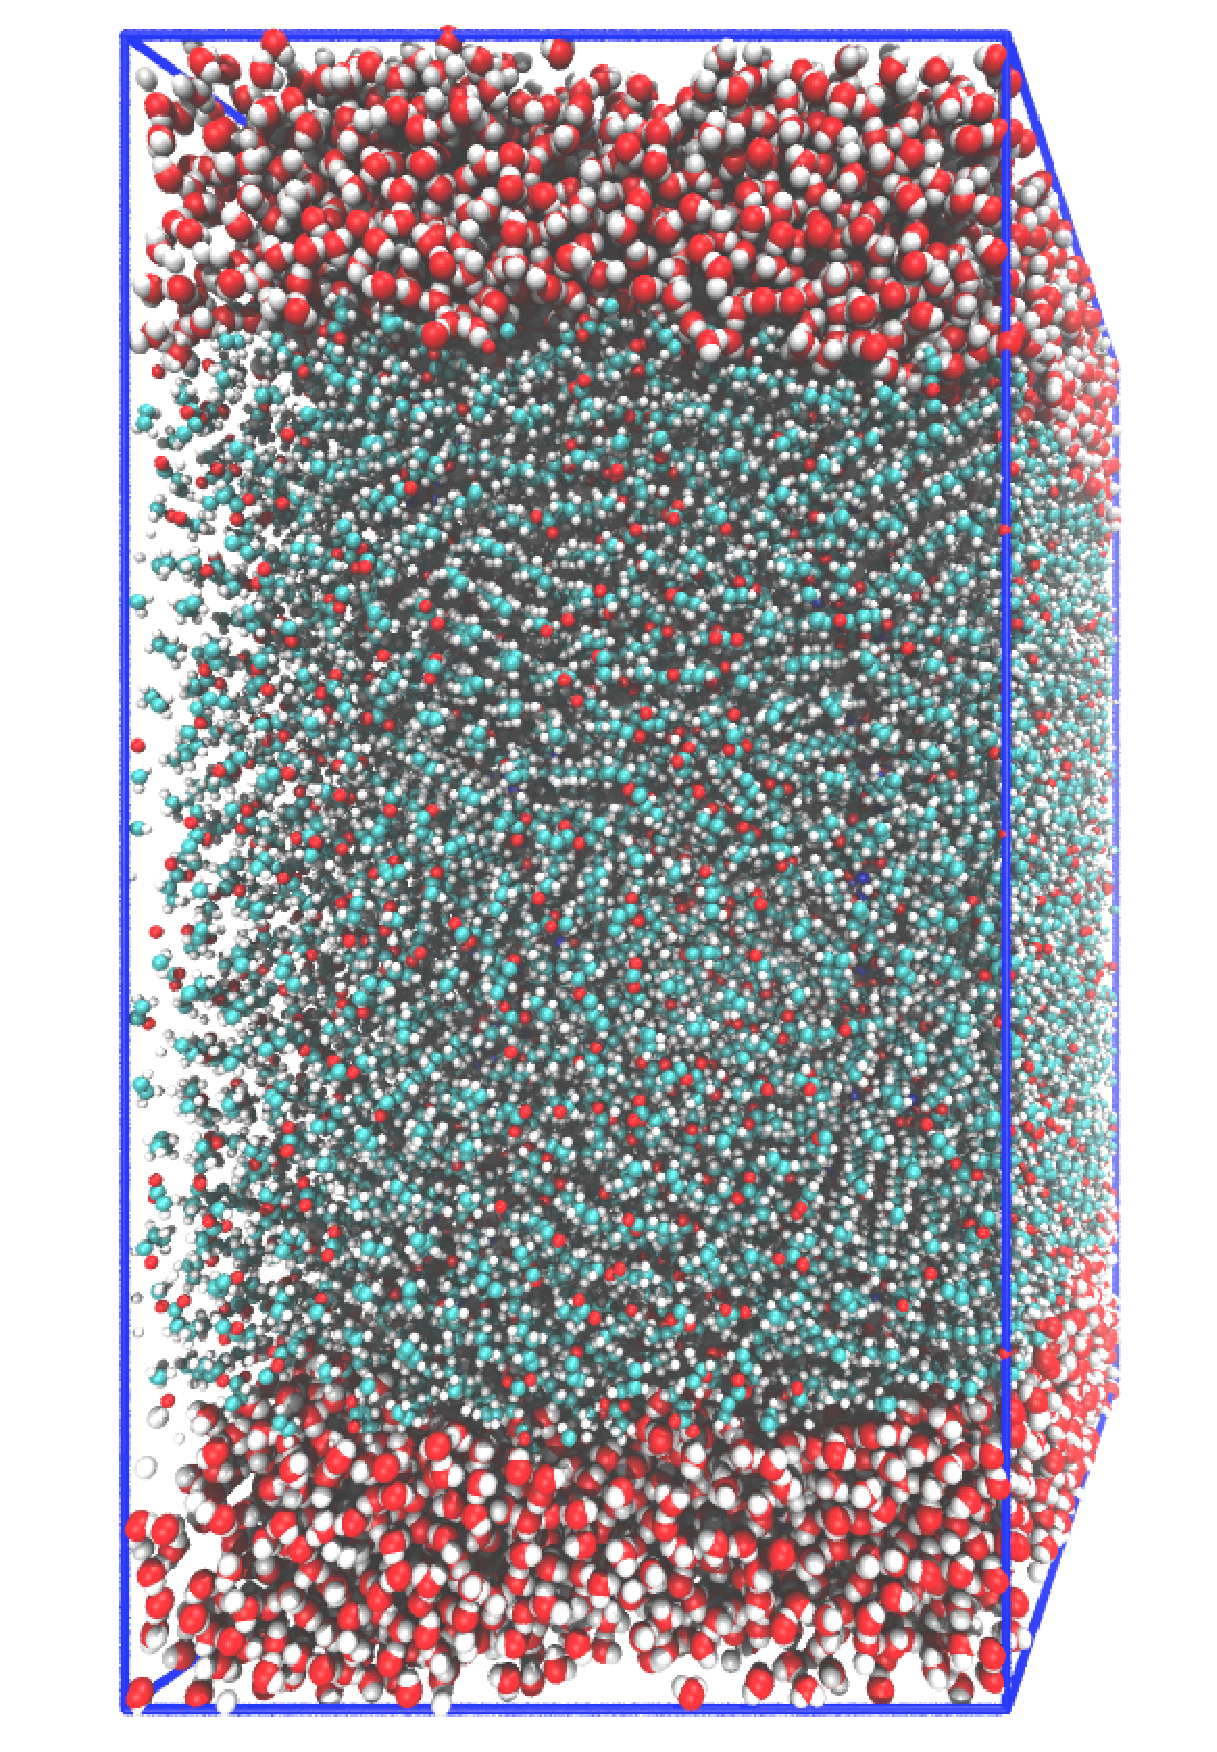
\includegraphics[width=\linewidth]{gap.pdf}
  \caption{}\label{fig:gap}
  \end{subfigure}  
  \begin{subfigure}{0.37\textwidth}
% Generated with : solute_partitioning.py -t shifted.xtc -g berendsen.gro -buffer 2 -r SOL
% in directory : /home/bcoscia/Documents/Gromacs/equilibration/solvation_equilibration/NaGA3C11/gaps/pre_equilibrated
  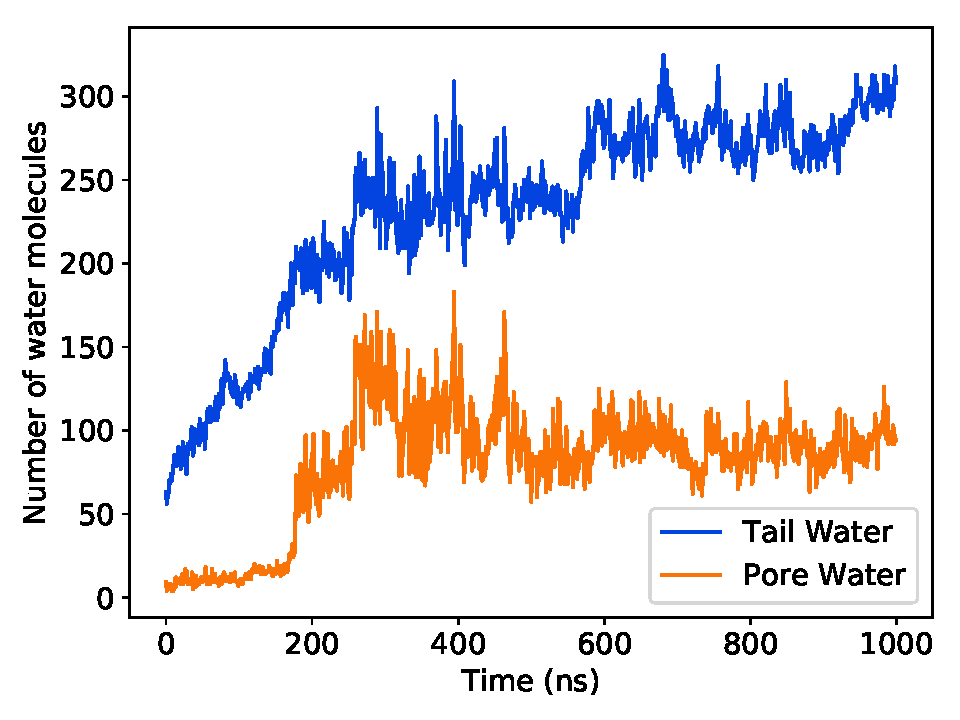
\includegraphics[width=\linewidth]{equilibrated_water_penetration.pdf}
  \caption{}\label{fig:equilibrated_water_penetration}
  \end{subfigure}  
  \begin{subfigure}{0.37\textwidth}
% Generated with custom script density.py located in same directory as above.
  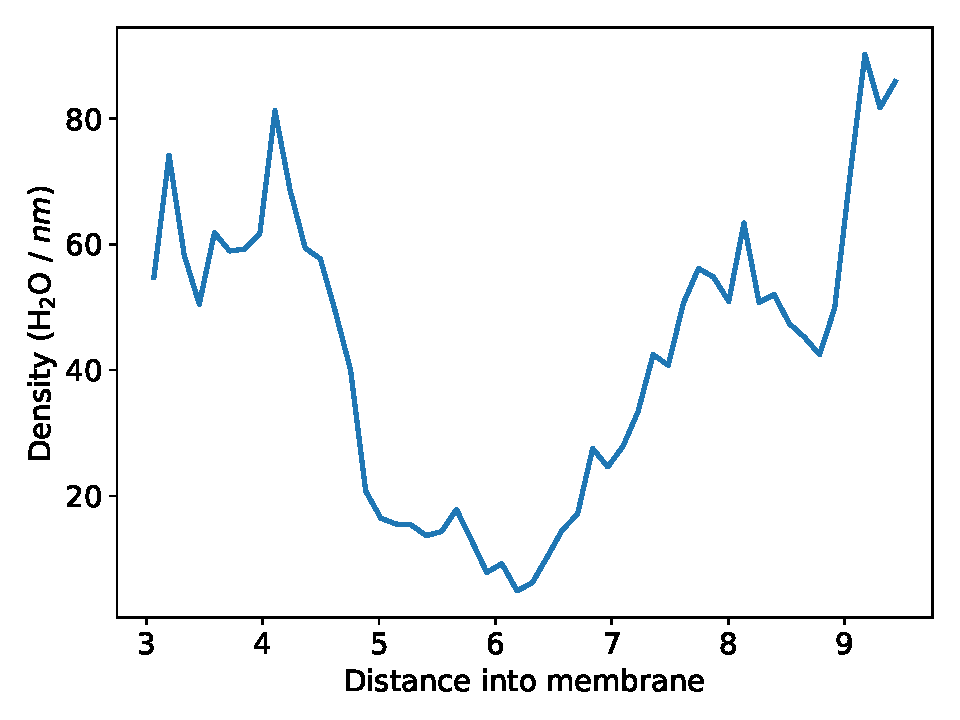
\includegraphics[width=\linewidth]{penetration_density.pdf}
  \caption{}\label{fig:penetration_density}
  \end{subfigure}  
  \caption{(a) Using an equilibrated dry configuration, we inserted a layer of water between
           periodic copies of the system in the $z$-direction. (b) Water slowly enters 
	   the membrane. Most water enters the tail region where the density of monomers is
	   lowest. Water entering the pore plateaus after 500 ns. (c) Although the water
	   content of the pore appears equilibrated in (b), the density of water throughout
	   the pores is not uniform, with almost no water close to the pore center. Note that
           the density is not shown below 3 nm or above 9.5 nm, because the the system
	   enters the water layer at those points.
  }\label{fig:gap_solvation}
  \end{figure}

  We equilibrated 4 systems where we initially placed water in the pores and in
  the tails in addition to a water reservoir between periodic images. We filled
  the pores with water by running \texttt{gmx solvate} on our initial
  configuration and removing any water molecules placed outside of the pore
  region. The GROMACS command \texttt{gmx solvate} places water molecules in
  proximity to other atoms based on their van der waals radii and therefore does
  a decent job of preventing equilibration issues. This also means that the
  intial pore radius dictates the water content of the pore. We can however, put
  arbitrary amounts of water into the tail region. We chose to test systems with
  initial pore radii of 5, 6, 7 and 8 \AA~with tail and pore water compositions
  given in Table~\ref{table:water_content}.

  \begin{table}[!htb]
  \centering
  \begin{tabular}{|c|c|c|}
  \hline
  Pore Radius (\AA) & wt \% water tails & wt \% water pores \\
  \hline
  5                 &        5.67       &     1.09          \\
  6                 &        2.88       &     2.38          \\
  7                 &        1.91       &     4.12          \\
  8                 &        2.78       &     6.00          \\
  \hline
  \end{tabular}
  \caption{We chose a diverse combination of initial pore and tail water
	  contents in order to study its effect on equilibrium water
	  content.}\label{table:water_content}
  \end{table}

  Systems appear to be most stable when there is more water in the pores than
  tails. In systems started with more water in the tails
  (Figures~\ref{fig:r5_gap} and \ref{fig:r6_gap}), the pore water content tends
  to increase over time, while that of the tails decreases or stays stable.
  Filling the pores with water is likely a very long process since it requires
  monomers to make space for water molecules. Systems started with a higher pore
  water content (Figures~\ref{fig:r7_gap} and \ref{fig:r8_gap}) tend to plateau
  relatively quickly, with about one third of the water staying in the tails.  We
  used this ratio in order to construct the initial configurations used for the
  studies in the main text.  Clearly, a more complicated methodology is needed in
  order to predict the equilibrium water content of a given LLC membrane.
  However, getting the value exactly right is not required for our study.
  Instead, we can observe mechanisms as a function of water content in each
  region. 

  \begin{figure}[!htb]
  \centering
  \begin{subfigure}{0.45\textwidth}
% Generated by running: solute_partitioning.py -t stabilized.xtc -g PR.gro -buffer 3 --savename water_partition.pl
% In directory: /home/bcoscia/Documents/Gromacs/equilibration/solvation_equilibration/NaGA3C11/water_content_experiments/5/1.09_5.67
  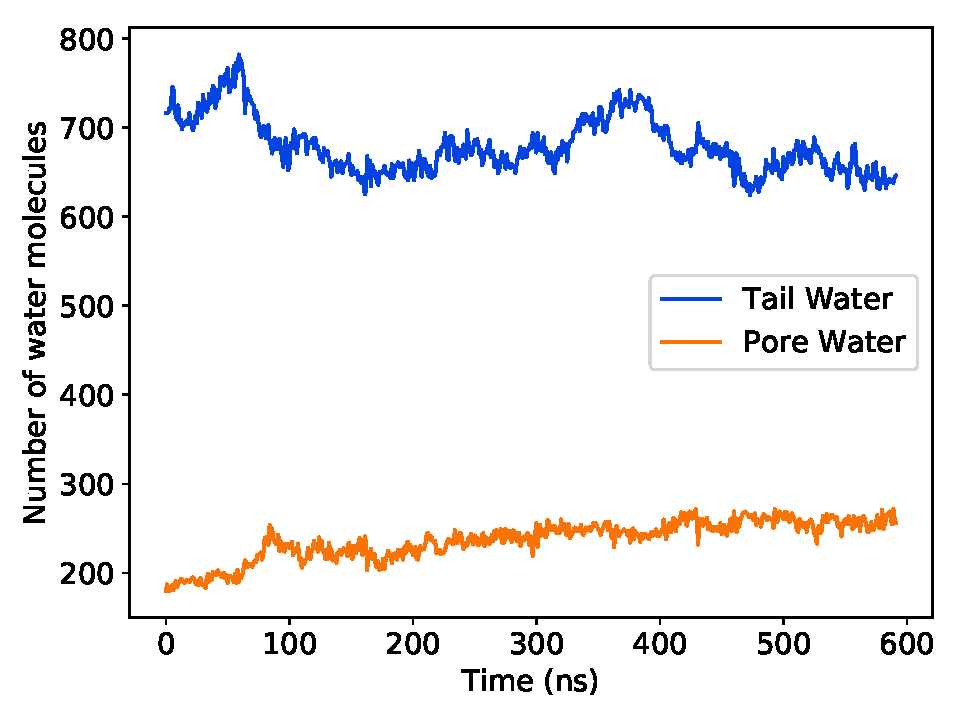
\includegraphics[width=\linewidth]{r5_gap.pdf}
  \caption{r = 5~\AA}\label{fig:r5_gap}
  \end{subfigure}
  \begin{subfigure}{0.45\textwidth}
% Generate by running: solute_partitioning.py -t stabilized.xtc -g PR.gro -buffer 2.5 -r SOL --savename water_partition.pl
% In directory: /home/bcoscia/Documents/Gromacs/equilibration/solvation_equilibration/NaGA3C11/water_content_experiments/6/2.38_2.88
  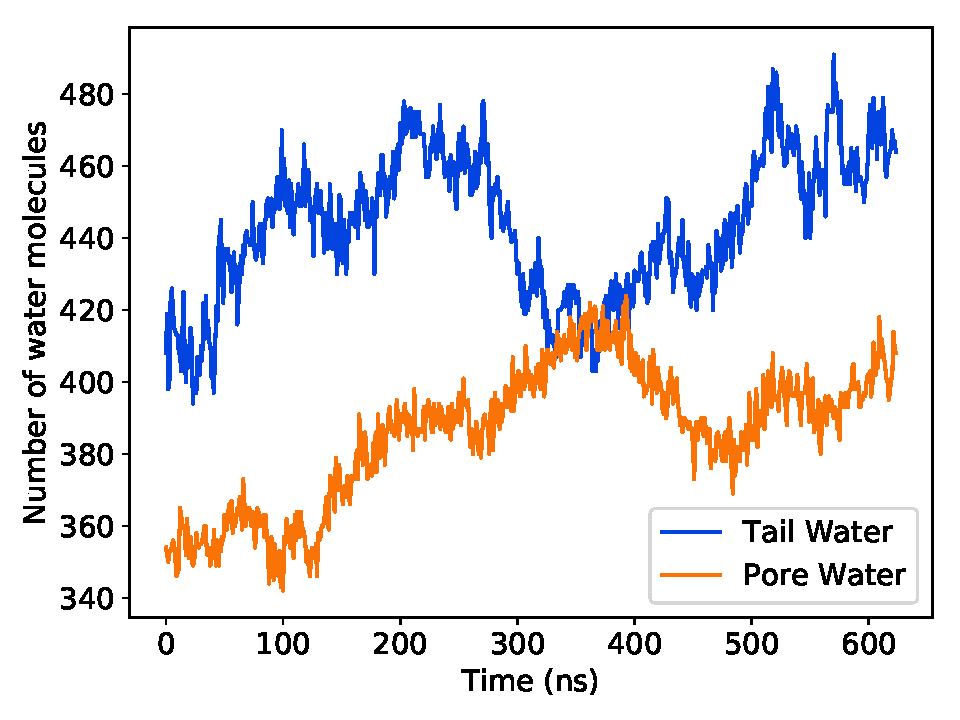
\includegraphics[width=\linewidth]{r6_gap.pdf}
  \caption{r = 6~\AA}\label{fig:r6_gap}
  \end{subfigure}
  \begin{subfigure}{0.45\textwidth}
% Generate by running: solute_partitioning.py -t stabilized.xtc -g last.gro -buffer 3 -r SOL --savename water_partition.pl
% In directory: /home/bcoscia/Documents/Gromacs/equilibration/solvation_equilibration/NaGA3C11/water_content_experiments/6/4.12_1.91
  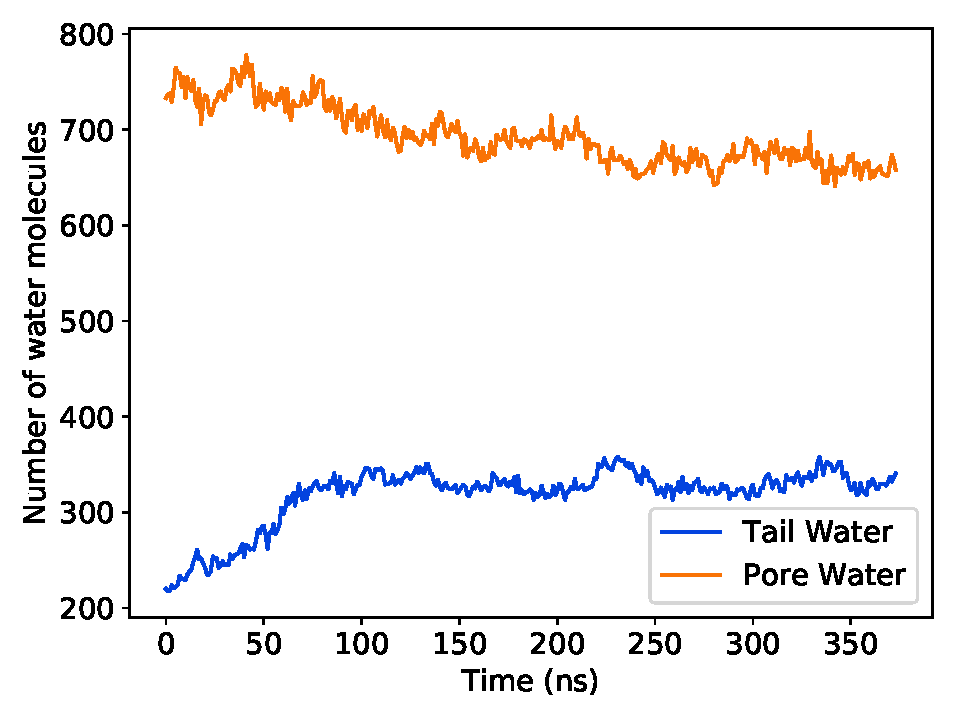
\includegraphics[width=\linewidth]{r7_gap.pdf}
  \caption{r = 7~\AA}\label{fig:r7_gap}
  \end{subfigure}
  \begin{subfigure}{0.45\textwidth}
% Generate by running: solute_partitioning.py -t stabilized.xtc -g last.gro -buffer 3 -r SOL --savename water_partition.pl
% In directory: /home/bcoscia/Documents/Gromacs/equilibration/solvation_equilibration/NaGA3C11/water_content_experiments/8/6.00_2.78
  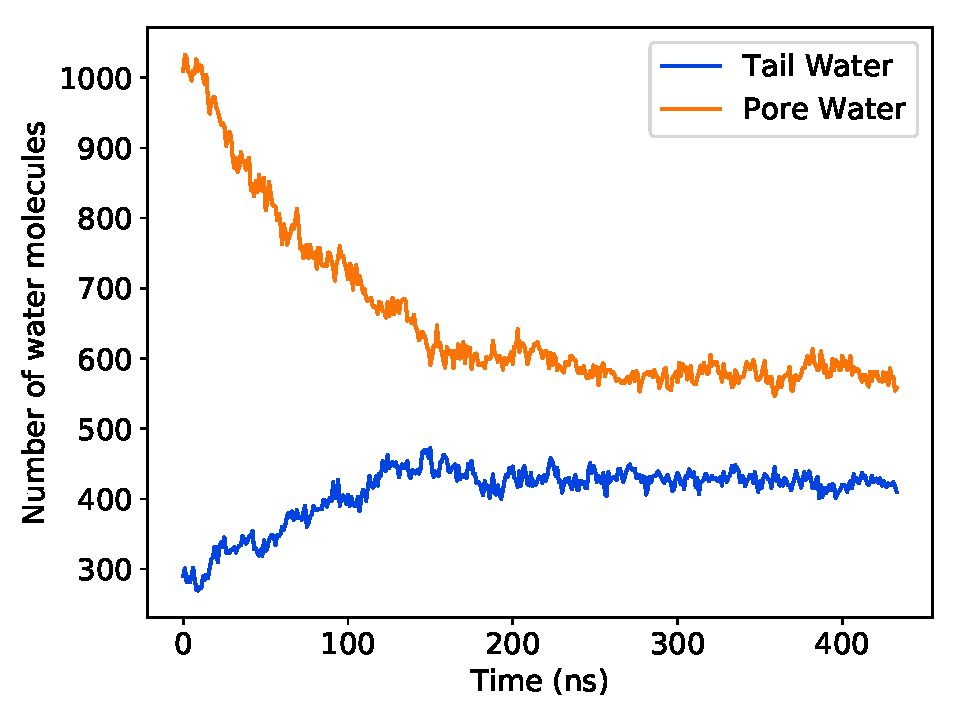
\includegraphics[width=\linewidth]{r8_gap.pdf}
  \caption{r = 8~\AA}\label{fig:r8_gap}
  \end{subfigure}
  \caption{There is likely more water in the pore region than in the tail region.
  When we create configurations with more water in the tails, equilibration is 
  slow. When configurations start with more water in the pores, the water content
  in each region equilibrates quickly.}\label{fig:gap_prefilled_equil}
  \end{figure}

  Since the equilibrium water content is unclear based on the previous
  simulations, we elected to choose and study systems with two different water
  contents. We removed the water reservoir and allowed the pore and tail water
  contents to equilibrate with 5 and 10 wt \% total water. We placed one third of
  the total water needed in the tails, based on the intuition gained in
  Figure~\ref{fig:gap_prefilled_equil}. We considered the water content
  equilibrated once the water contents plateaued. The 5 wt\% system did
  not plateau until $\sim$ 600 ns (Figure~\ref{fig:5wt_offset_equil})
  while the 10 wt \% water system equilibrated within the first 100 ns of 
  simulation (Figure~\ref{fig:10wt_offset_equil}).
  The pores contain 72 \% and 69 \% of the total water in the 5 and 10 wt \%
  systems respectively.

  \begin{figure}
  \centering
  \begin{subfigure}{0.45\textwidth}
% Generated with solute_partitioning.py -t full_shifted.xtc -g berendsen.gro -r SOL -pr 1.6 --savename water_partitioning.pl
% in directory /home/bcoscia/Documents/Gromacs/equilibration/solvation_equilibration/NaGA3C11/offset/5wt
  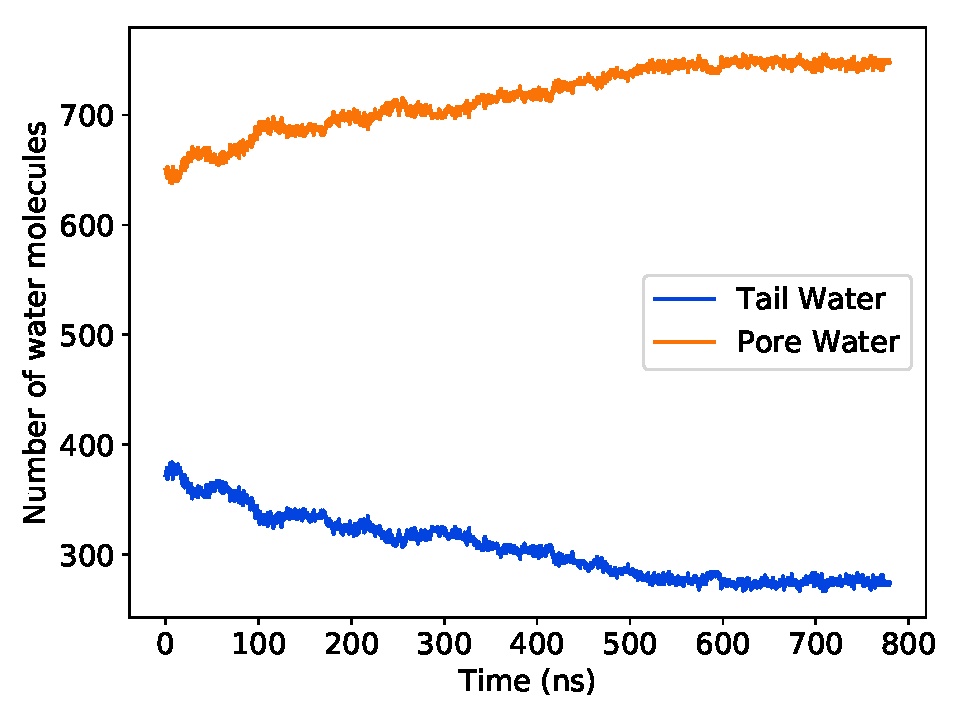
\includegraphics[width=\textwidth]{5wt_offset_equil.pdf}
  \caption{5 wt \%}\label{fig:5wt_offset_equil}
  \end{subfigure}
  \begin{subfigure}{0.45\textwidth}
  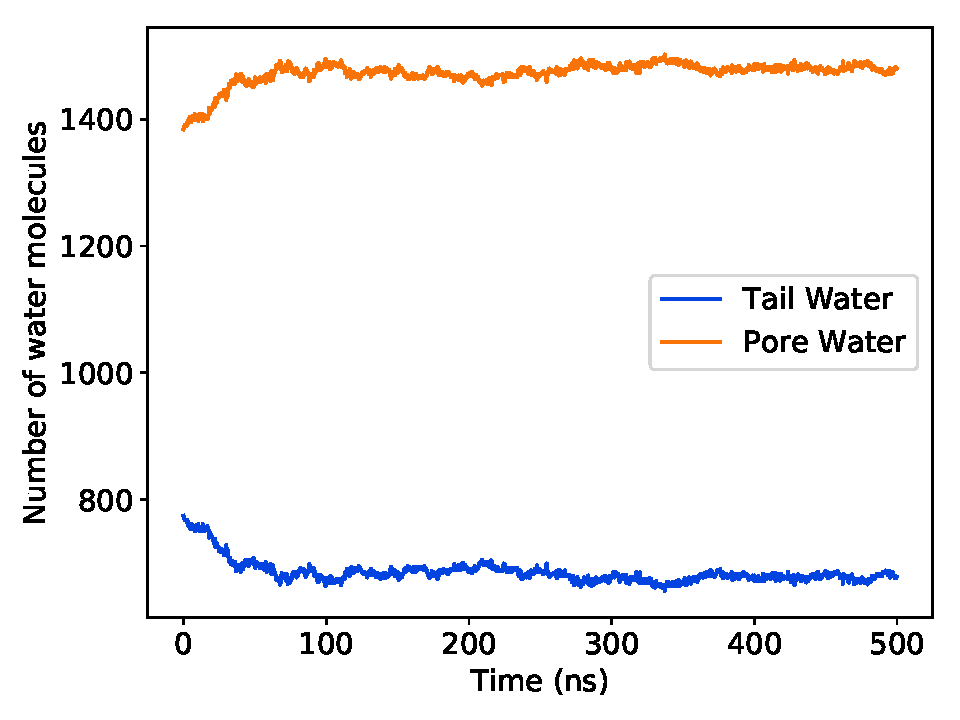
\includegraphics[width=\textwidth]{10wt_offset_equil.pdf}
  \caption{10 wt \%}\label{fig:10wt_offset_equil}
% Generated with solute_partitioning.py -t shifted.xtc -g last.gro -r SOL -pr 1.48 --savename water_partitioning.pl
% in directory /home/bcoscia/Documents/Gromacs/equilibration/solvation_equilibration/NaGA3C11/offset/10wt
  \end{subfigure}
  \caption{We created solvated systems with one third of the total water
	  initially placed in the tail region. (a) With 5 wt \% total water, the water
	  content equilibrates after 600 ns, with $\sim$ 72 \% of the total water in the
	  pores. (b) With 10 wt \% total water, the water content equilibrates after 100
	  ns, with $\sim$ 69 \% of the total water in the
	  pores.}\label{fig:solvation_equilibration}
  \end{figure}

  We cross-linked the equilibrated solvated systems, then allowed them to 
  equilibrate further for 100 ns. The water contents in each region does not
  change significantly in either case.

  \begin{figure}
  \centering
  \begin{subfigure}{0.45\textwidth}
% Generated with solute_partitioning.py -t PR.trr -g PR.gro -r SOL --savename SOL_partitioning.pl
% In directory /home/bcoscia/Documents/Gromacs/equilibration/xlink_equilibration/NaGA3C11/5wt
  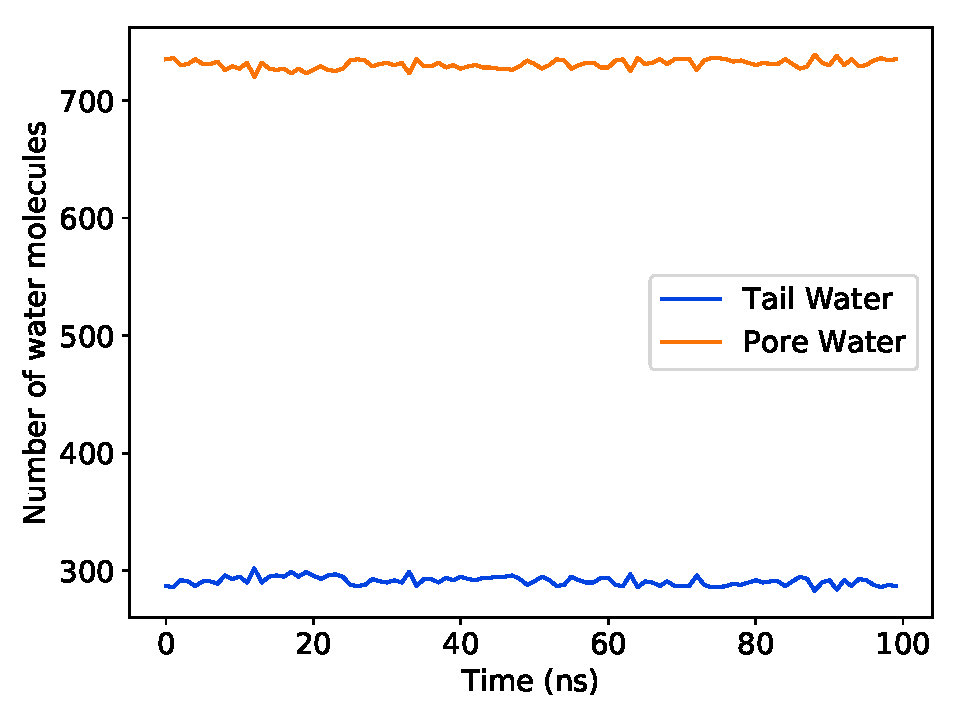
\includegraphics[width=\textwidth]{5wt_offset_xlinked_equil.pdf}
  \caption{5 wt\%}\label{fig:5wt_offset_xlinked_equil}
  \end{subfigure}
  \begin{subfigure}{0.45\textwidth}
  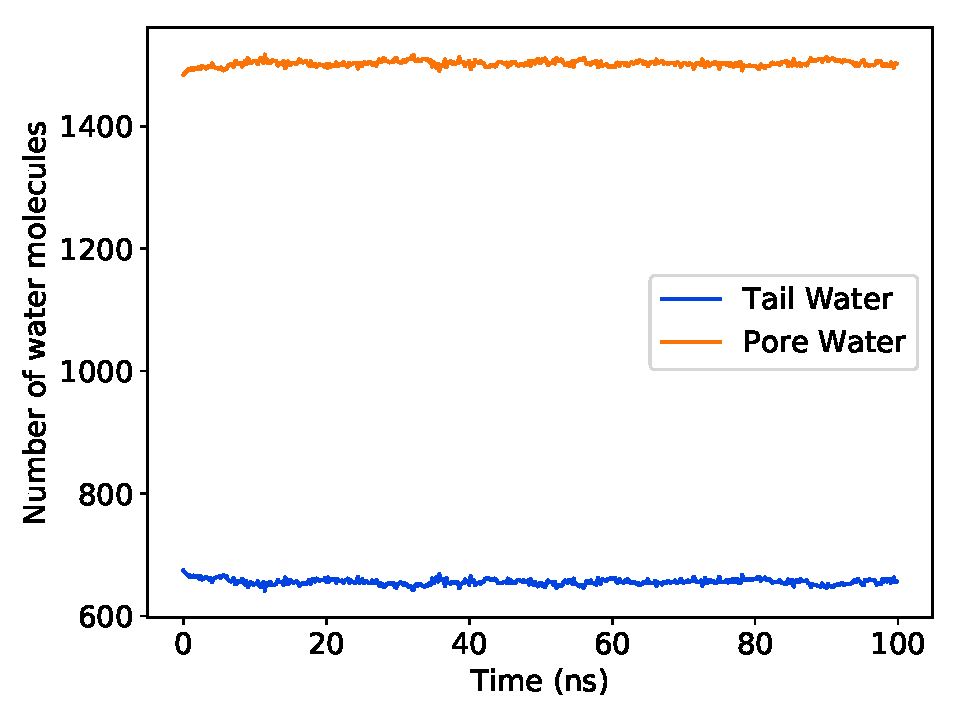
\includegraphics[width=\textwidth]{10wt_offset_xlinked_equil.pdf}
  \caption{10 wt\%}\label{fig:10wt_offset_xlinked_equil}
% Generated with solute_partitioning.py -t xlinked_equil.trr -g xlinked_equil.gro -r SOL -pr 1.48 --savename water_partitioning.pl
% In directory /home/bcoscia/Documents/Gromacs/equilibration/xlink_equilibration/NaGA3C11/10wt/63_percent
  \end{subfigure}
  \caption{The water content in the tail and pore region is not affected
  by cross-linking}\label{fig:solvation_equilibration}
  \end{figure}
  
  \subsection{Solute Interaction}\label{section:solute_interaction}
  
  We chose to model 6 solutes in each pore because there was a low degree of 
  interaction between solutes which gave us a sufficient number of independent 
  trajectories to observe and analyze. There are a negligible number of occurrences
  % BJC: not sure what the appropriate cut-off should be
  where the center of a given solute came within 3.5 \AA of another same-solute
  center of mass.
  
  \begin{figure}
  \centering
  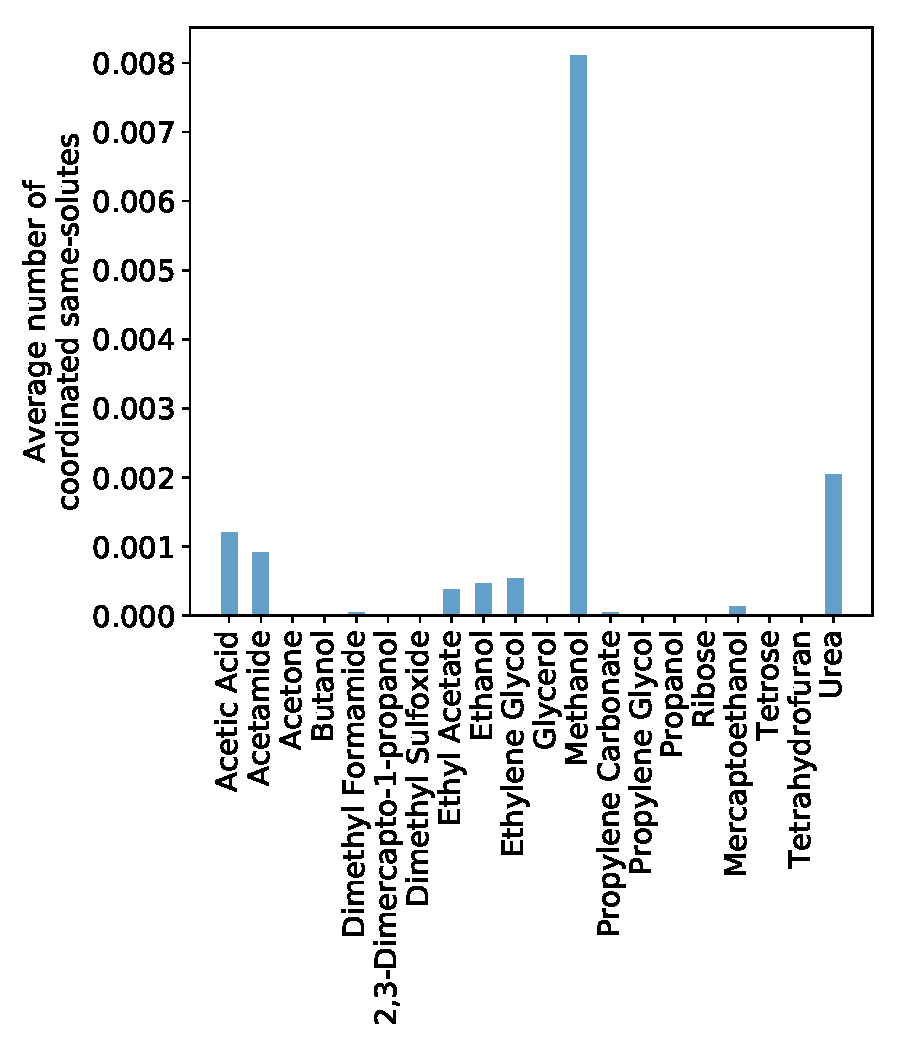
\includegraphics[width=0.45\textwidth]{solute_interaction.pdf}
  \caption{Interactions between same-solutes are negligible when systems are 
  built with 6 solutes per pore. Even methanol, which interacts with other same-solute
  molcules the most, does so less than 0.05 \% of the time.}\label{fig:solute_interation}
  \end{figure}

% BJC: the arguments in the following section aren't as strong as I want them to be. 
% And not necessary for this paper.
%
%  \section{Choosing a transport model}\label{section:transport_model_selection}
%
%  We used the toolbox created by Meroz and Sokolov in order to justify our
%  choice of transport model.\cite{meroz_toolbox_2015} The solutes in our systems
%  exhibit anomalous transport properties characteristic of a Continuous Time
%  Random Walk (CTRW). 
%
%  \subsection*{Mean Squared Displacement}
%
%  The general form of a mean squared displacement (MSD) curve is:
%  \begin{equation}
%	\langle x^2(t) \rangle \sim t ^ \alpha
%	\label{eqn:msd}
%  \end{equation}
%  For brownian motion, $\alpha = 1$ and the MSD is linear. When $\alpha \neq
%  1$, the particle of interest exhibits anomalous diffusion. Values of $\alpha$
%  greater than 1 give rise to superdiffusion, while values of $\alpha$ less than
%  1 give rise to subdiffusion.
%
%  We can calculate the ensemble-averaged MSD curve by averaging the MSDs of
%  each particle trajectory, where each MSD is calculated using:
%  \begin{equation}
%	\delta^2(t) = \| \mathbf{r}(t) - \mathbf{r}(0) \|^2
%	\label{eqn:ensemble_msd}
%  \end{equation}
%  where $\|\cdot\|$ represents the Euclidean norm. 
%
%  The mean squared displacement of solutes in our model is a non-linear
%  function of time, with $\alpha < 1$ which is indicative of anomalous
%  subdiffusion. Figure \ref{fig:msd_power_law}a plots the ensemble-averaged MSD
%  curve for 24 ethanol molecules diffusing in a 10 wt\% water H\textsubscript{II}
%  LLC membrane system. We fit a power law of the form $Ae^{\alpha}$ to the MSD
%  curve. We performed 2000 bootstrap trials by randomly sampling 24 MSD curves
%  with replacement from the 24 total ethanol MSD curves. The bootstrapped average
%  value of $\alpha$ is 0.75 for this system. 
% 
%  \begin{figure}[!htb]
%  \centering
%% Generated with : msd.py -t PR_nojump.xtc -g PR.gro -r ETH -ensemble -power_law -a z -nboot 2000
%% in directory: /home/bcoscia/Documents/Gromacs/Transport/NaGA3C11/ETH/10wt
%  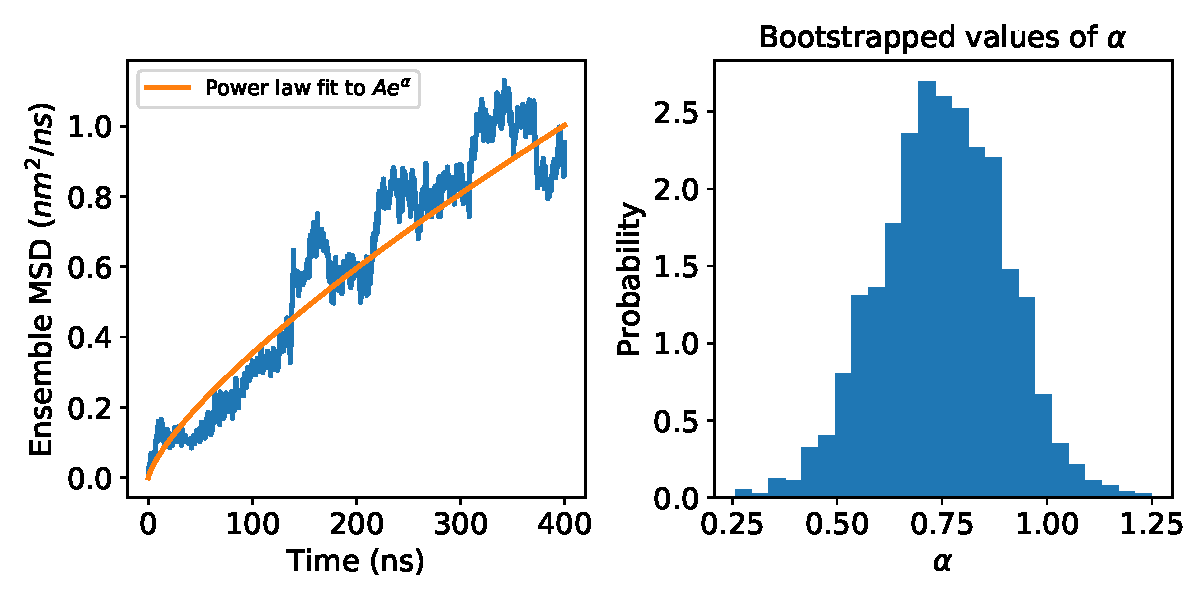
\includegraphics[width=0.8\linewidth]{msd_power_law.pdf}
%  \caption{(a) We fit a curve with the form of Equation~\ref{eqn:msd} to the
%	  ensemble-averaged MSD curve. (b) The average value of $\alpha$, obtained using
%	  fits to MSDs calculated from bootstrapped ensembles, is less than 1 suggesting
%	  that ethanol molecules in our model exhibit subdiffusive
%	  behavior.}\label{fig:msd_power_law}
%  \end{figure}
%
%  \subsection*{Ergodicity}
%
%  The ergodicity of a system can help us narrow down the possible anomalous
%  diffusion mechanisms. In an ergodic system, the time-averaged behavior of an
%  observable should yield the same result as the ensemble average of the same
%  observable. Examples of anomalous diffusion processes that are ergodic include
%  random walks on fractals (RWF) and fractional brownian motion (FBM).
%  Non-ergodic systems generally give rise to CTRWs with the possibility of
%  combination with a RWF and/or FBM.\cite{meroz_toolbox_2015} 
%
%  We tested the ergodicity of our system by comparing the ensemble-averaged
%  and time-averaged MSD curves. We calculated the MSD of each ethanol trajectory
%  using Equation~\ref{eqn:ensemble_msd} and a time-averaged algorithm: 
%  \begin{equation}
%	\delta^2(t) = \dfrac{1}{N-t} \sum_{i=0}^{N-t-1} \| \mathbf{r}(i + t) - \mathbf{r}(i) \|^2
%  \end{equation}
%  where N is the total number of simulation frames, and t represents the length
%  of subinterval or number of frames per subinterval. We averaged the MSD curves
%  from each trajectory in order to create final MSD plots.
%
%  The ethanol molecules exhibit non-ergodic behavior because their
%  time-averaged and ensemble-averaged MSDs do not agree with each other
%  (Figure~\ref{fig:ethanol_msd_comparison}). We validated our analysis using a 1
%  ns simulation of a box of tip3p water molecules. As expected, since the
%  particles exhibit Brownian motion, the time-averaged and ensemble-averaged MSDs
%  agree with each within error (Figure~\ref{fig:water_box_msd_comparison}).
%
%  \begin{figure}[!htb]
%  \centering
%  \begin{subfigure}{0.45\textwidth}
%% Generated with : msd.py -t PR_nojump.xtc -g PR.gro -r ETH -compare -nboot 2000 -a z
%% in directory: /home/bcoscia/Documents/Gromacs/Transport/NaGA3C11/ETH/10wt
%  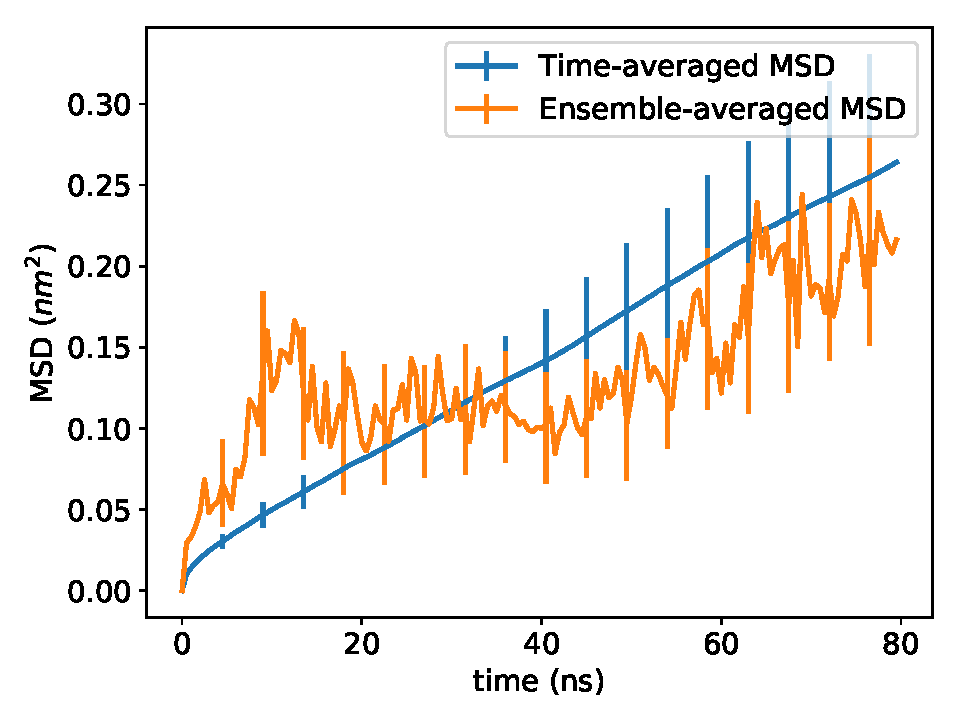
\includegraphics[width=\textwidth]{ethanol_msd_comparison.pdf}
%  \caption{}\label{fig:ethanol_msd_comparison}
%  \end{subfigure} 
%  \begin{subfigure}{0.45\textwidth}
%% Generated with msd.py -t traj_nojump.xtc -g npt.gro -r SOL -compare --fracshow 0.4 -nboot 2000 -a z
%% in directory: /home/bcoscia/Documents/Gromacs/Transport/Solvent/solvent_boxes/pure_water
%  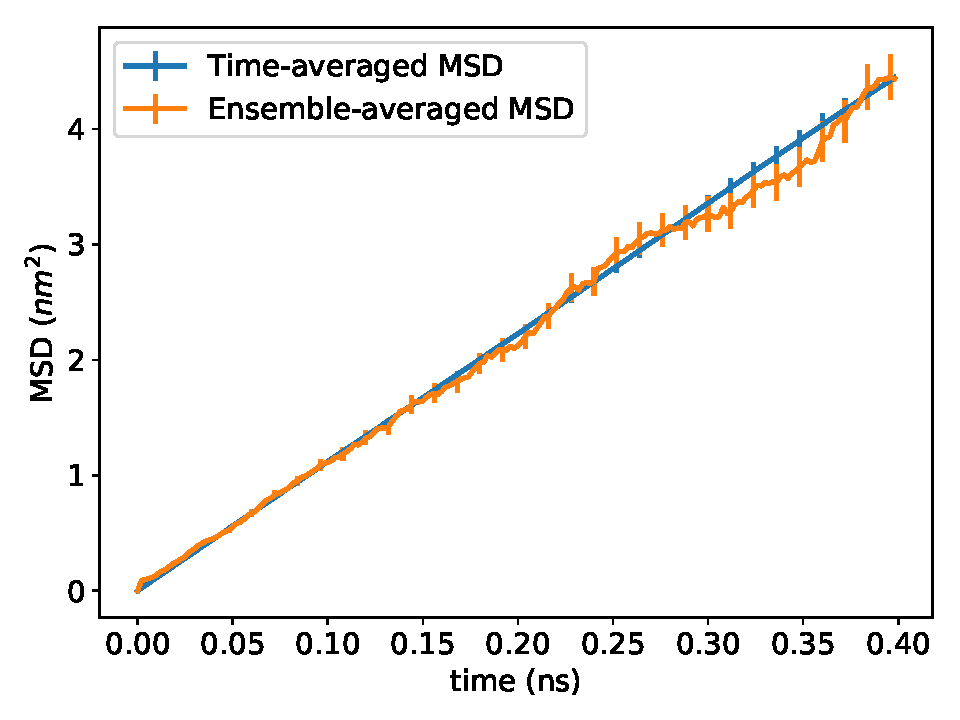
\includegraphics[width=\textwidth]{water_box_msd_comparison.pdf}
%  \caption{}\label{fig:water_box_msd_comparison}
%  \end{subfigure} 
%  \caption{(a) The time-averaged and the ensemble-averaged MSDs for ethanol in
%	  an H\textsubscript{II} nanopore are not in agreement, implying non-ergodicity.
%	  (b) A box of tip3p water molecules is expected to be ergodic and it is shown to
%	  be true here because both MSDs are in agreement. }\label{fig:msd_comparison}
%  \end{figure}
%
%  \subsection*{Autocorrelation of steps}
%
%% From Sokolov paper: "Assigning different waiting times τ i to each step, and assuming that the
%% steps are uncorrelated as in a regular RW, gives rise to the CTRW model" -- I
%% might need to check autocorrelation of steps lengths when a hop occurs rather
%% than every time step. Not sure if there is enough data for that, but could check 
%% a particularly hoppy trajectory after longer simulation.
%
%
%  Based on the previous two sections, our model can likey be studied as a CTRW. 
%  However, it is still possible that our CTRW model might also be convoluted with
%  an FBM or a RWF process. In a pure CTRW, the steps are uncorrelated. 
%  Both FBM and RWF exhibit anti-correlated steps. 
%
%  The steps in our system are not correlated. We showed this by calculating the
%  autocorrelation function (ACF) of the step lengths in the $z$-direction. The
%  ACF of a representative trajectory is shown in Figure~\ref{fig:eth_autocorrelation}.  
%  
%  \begin{figure}[!htb]
%  \centering
%% Generated with brownian_test.py -t PR_nojump.xtc -g PR.gro -r ETH (and appropriate uncommenting -- need to rework that script)
%% in directory: /home/bcoscia/Documents/Gromacs/Transport/NaGA3C11/ETH/10wt
%  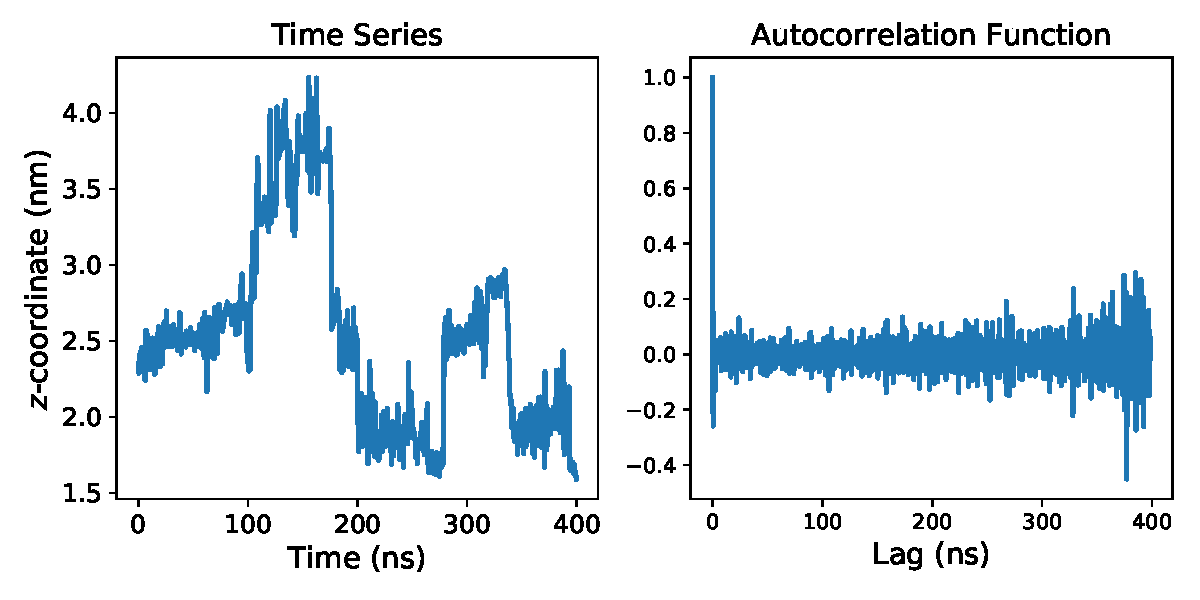
\includegraphics[width=0.8\textwidth]{eth_autocorrelation.pdf}
%  \caption{The autocorrelation function (right) of a representative ethanol
%	   center of mass $z$-coordinate trajectory (left) almost immediately decays to zero,
%	   indicating a complete loss of memory of it's previous position. Noise increases
%	   at large time lags due to decreased sampling.}\label{fig:eth_autocorrelation}
%  \end{figure}

  \clearpage
  \bibliography{transport}

\end{document}
